\documentclass[12pt,a4paper]{report}
\usepackage[utf8]{inputenc}
\usepackage[T1]{fontenc}
\usepackage[french]{babel}
\usepackage{graphicx}
\usepackage{geometry}
\usepackage{hyperref}
\usepackage{fancyhdr}
\usepackage{titlesec}
\usepackage{setspace}
\usepackage{tcolorbox}
\usepackage{booktabs}
\usepackage{float}
\usepackage{caption}

\geometry{top=2.5cm, bottom=2.5cm, left=2.5cm, right=2.5cm}
\onehalfspacing

% Stylisation des titres
\titleformat{\chapter}[display]
  {\normalfont\huge\bfseries\color{black}}{\chaptertitlename\ \thechapter}{20pt}{\Huge}
\titlespacing*{\chapter}{0pt}{-50pt}{40pt}

% En-tête et pied de page
\pagestyle{fancy}
\fancyhf{}
\fancyhead[L]{Plateforme Intelligente d'Assistance Académique}
\fancyhead[R]{ENSA Tétouan}
\fancyfoot[C]{\thepage}

\begin{document}

\begin{titlepage}
    \centering
    
\includegraphics[width=6cm]{logo.png}\\[1cm] % Logo placeholder
    
    {\large \textbf{Ecole Nationale des Sciences Appliquées de Tétouan}}\\[1.5cm]
    
    {\Large \textbf{RAPPORT DE PROJET}}\\[2cm]
    
    \rule{\linewidth}{0.5mm} \\[0.5cm]
    {\huge \textbf{Plateforme Intelligente d'Assistance Académique Basée sur l'Intelligence Artificielle}} \\[0.5cm]
    \rule{\linewidth}{0.5mm} \\[2.5cm]
    
    \begin{minipage}{0.45\textwidth}
        \begin{flushleft} \large
            \textbf{Réalisé par :}\\
            \vspace{0.2cm}
            SOULAMA Doubie Judicael Noé \textit{(Big Data et IA)}\\
            YASSIR Moussa \textit{(Cybersécurité)}\\
            DAO Ambdou Rafiou \textit{(Cybersécurité)}\\
            OWUSU Justin Afful \textit{(Génie Civil)}
        \end{flushleft}
    \end{minipage}
    \hfill
    \begin{minipage}{0.45\textwidth}
        \begin{flushright} \large
            \textbf{Encadré par :} \\
            M. BEN KASMIA NIZAR \\
        \end{flushright}
    \end{minipage}
    
    \vfill
    {\large Année universitaire : 2025 -- 2026}
\end{titlepage}

\chapter*{Résumé}
\addcontentsline{toc}{chapter}{Résumé}
Avec l'évolution des technologies numériques, les universités cherchent à améliorer l'accès aux ressources pédagogiques et à faciliter l'accompagnement des étudiants. Dans ce projet, nous proposons la conception d'une plateforme intelligente d'assistance académique basée sur l'intégration de technologies web modernes et de l'intelligence artificielle.

L'objectif principal est de développer un système capable d'aider les étudiants dans leur apprentissage en leur proposant des outils tels que :
\begin{itemize}
    \item la génération automatique de quiz et d'exercices
    \item des recommandations de révision personnalisées
    \item l'analyse des performances académiques.
\end{itemize}
Cette plateforme permettra également aux enseignants de suivre plus facilement la progression des étudiants.

\tableofcontents

\chapter{Introduction}
\section{Contexte général}
Les établissements universitaires jouent un rôle fondamental dans la formation des étudiants et dans le développement des compétences nécessaires au monde professionnel. Cependant, avec l'augmentation constante du nombre d'étudiants et la complexification des parcours académiques, les universités doivent aujourd'hui faire face à de nouveaux défis en matière de gestion administrative et d'accompagnement pédagogique.

Malgré les progrès importants réalisés dans le domaine des technologies de l'information et de la communication, de nombreuses universités continuent d'utiliser des systèmes administratifs et pédagogiques relativement traditionnels. Ces systèmes reposent encore souvent sur des processus manuels ou semi-numériques qui peuvent ralentir certaines procédures et limiter l'efficacité des services proposés aux étudiants.

Par ailleurs, les besoins des étudiants évoluent rapidement. Les étudiants d'aujourd'hui sont de plus en plus habitués à utiliser des outils numériques intelligents capables de leur fournir des informations rapidement et de manière personnalisée. Dans ce contexte, les universités doivent repenser leurs systèmes afin de proposer des solutions plus modernes, plus efficaces et mieux adaptées aux attentes des utilisateurs.

L'émergence de technologies telles que l'intelligence artificielle offre aujourd'hui de nouvelles opportunités pour améliorer la gestion universitaire et proposer des services innovants capables d'accompagner les étudiants tout au long de leur parcours académique.

\section{Constats principaux}
Dans de nombreux établissements universitaires, plusieurs difficultés persistent encore au niveau administratif et pédagogique.

Tout d'abord, les procédures administratives restent souvent longues et complexes. Les étudiants doivent généralement se rendre physiquement dans différents services pour effectuer certaines démarches administratives, comme la demande de documents officiels, la validation de dossiers ou encore l'obtention d'attestations.

Ensuite, l'obtention de documents administratifs peut prendre plusieurs jours, voire plusieurs semaines, ce qui peut retarder certaines démarches importantes pour les étudiants, notamment dans le cadre de stages, de candidatures ou de procédures administratives externes.

De plus, les services administratifs sont fréquemment confrontés à un grand nombre de demandes simultanées, ce qui entraîne souvent la formation de longues files d'attente et une surcharge de travail pour le personnel administratif.

Au niveau académique, les étudiants rencontrent également plusieurs difficultés. Beaucoup d'entre eux ont du mal à organiser efficacement leurs révisions et à identifier les chapitres qu'ils doivent approfondir. Certains étudiants manquent également de repères pour évaluer leur niveau de préparation avant les examens.

Du côté des enseignants, il n'est pas toujours facile de disposer d'outils permettant d'analyser rapidement et précisément les performances des étudiants. Les enseignants doivent souvent se baser uniquement sur les résultats d'examens ou sur leur expérience personnelle pour identifier les chapitres les plus difficiles pour les étudiants.

Ces différents constats montrent qu'il existe un besoin réel d'outils numériques intelligents capables d'améliorer à la fois la gestion administrative et l'accompagnement pédagogique dans les universités.

\section{Présentation du projet}
Afin de répondre à ces différentes problématiques, ce projet propose la conception et le développement d'une plateforme numérique intelligente destinée à améliorer l'expérience universitaire des étudiants et des enseignants.

Cette plateforme prendra la forme d'un système accessible à la fois via une application web et une application mobile, permettant aux utilisateurs d'accéder facilement aux différents services proposés.

L'un des éléments centraux de cette solution repose sur l'intégration de fonctionnalités basées sur l'intelligence artificielle. Ces fonctionnalités permettront notamment d'automatiser certaines tâches administratives, d'accompagner les étudiants dans leur apprentissage et de fournir aux enseignants des outils d'analyse avancés.

La plateforme sera conçue comme un assistant académique et administratif intelligent, capable d'interagir avec les utilisateurs, de comprendre leurs besoins et de leur proposer des solutions adaptées. L'objectif est de créer un environnement numérique qui facilite l'accès aux services universitaires tout en améliorant la qualité de l'accompagnement pédagogique.

\section{Objectif général du projet}
L'objectif principal de ce projet est de concevoir une plateforme numérique intelligente capable d'améliorer le fonctionnement du système universitaire en combinant les technologies du numérique et de l'intelligence artificielle.

Plus précisément, cette plateforme devra permettre de simplifier certaines démarches administratives en offrant aux étudiants la possibilité de faire leurs demandes directement en ligne, sans avoir besoin de se déplacer physiquement dans les services administratifs.

Elle devra également accompagner les étudiants dans leur parcours académique en leur proposant des outils intelligents capables de les aider à mieux organiser leurs révisions, à comprendre les concepts difficiles et à évaluer leur niveau de préparation avant les examens.

Par ailleurs, la plateforme devra fournir aux enseignants des outils d'analyse permettant d'obtenir une vision plus claire des performances des étudiants, d'identifier les chapitres les plus complexes et d'adapter leurs méthodes pédagogiques en conséquence.

Ainsi, cette solution vise à créer un système plus efficace, plus interactif et plus adapté aux besoins actuels de l'enseignement supérieur.


\chapter{Problématique}
\section{Problèmes administratifs}
Dans de nombreuses universités, les procédures administratives reposent encore largement sur des méthodes traditionnelles qui peuvent être longues et inefficaces.

Les étudiants doivent souvent se déplacer physiquement pour effectuer certaines démarches administratives, telles que la demande d'attestations, la récupération de documents officiels ou la validation de certaines informations académiques.

La gestion des demandes se fait parfois de manière manuelle, ce qui peut entraîner des erreurs, des retards et une surcharge de travail pour le personnel administratif.
De plus, les délais de traitement peuvent être relativement longs, ce qui peut poser problème pour les étudiants qui ont besoin de certains documents dans des délais courts, notamment pour des démarches externes comme les candidatures à des stages ou à des programmes d'échange.

Enfin, les procédures administratives ne sont pas toujours clairement expliquées aux étudiants, ce qui peut entraîner des incompréhensions et des démarches répétées.

\section{Problèmes académiques}
Au niveau pédagogique, plusieurs difficultés peuvent également être observées. Certains étudiants rencontrent des difficultés pour comprendre certains concepts ou certains chapitres, en particulier dans les disciplines techniques ou scientifiques. L'absence d'un accompagnement personnalisé peut rendre l'apprentissage plus difficile pour certains profils d'étudiants.

De plus, les étudiants ne disposent pas toujours d'outils efficaces pour organiser leurs révisions. Ils peuvent avoir du mal à déterminer quels chapitres doivent être prioritaires ou à planifier leur temps de travail de manière optimale.

Par ailleurs, il est souvent difficile pour les étudiants d'évaluer leur niveau réel avant les examens. Beaucoup d'entre eux ne savent pas s'ils sont suffisamment préparés ou s'ils doivent encore approfondir certains sujets.

Ces difficultés montrent l'importance de développer des outils capables d'accompagner les étudiants de manière plus personnalisée.

\section{Limites du côté des enseignants}
Les enseignants rencontrent également certaines limites dans le suivi pédagogique des étudiants. Dans de nombreux cas, ils ne disposent pas d'outils analytiques leur permettant de suivre en détail les performances individuelles et collectives des étudiants.

Il peut également être difficile pour eux d'identifier rapidement les chapitres qui posent le plus de difficultés à l'ensemble de la classe. Cette information pourrait pourtant être très utile pour adapter les explications ou proposer des exercices supplémentaires.

De plus, les enseignants ne disposent pas toujours de systèmes permettant de générer automatiquement des analyses ou des rapports pédagogiques qui pourraient les aider à mieux comprendre l'évolution du niveau des étudiants au cours du semestre.

\section{Synthèse du problème}
À partir de ces différentes observations, il apparaît que le système universitaire actuel présente plusieurs limites importantes.

Premièrement, la gestion administrative reste relativement lente et peu automatisée. Deuxièmement, l'accompagnement académique proposé aux étudiants n'est pas toujours suffisamment personnalisé pour répondre aux besoins individuels. Troisièmement, les enseignants disposent de peu d'outils intelligents leur permettant d'analyser efficacement les performances des étudiants et d'adapter leurs méthodes pédagogiques.

Ces différentes limites montrent qu'il existe un réel potentiel d'amélioration grâce à l'utilisation de solutions numériques innovantes.

\section{Question centrale}
Dans ce contexte, la question centrale qui guide ce projet peut être formulée de la manière suivante :

\begin{tcolorbox}[colback=blue!5!white,colframe=blue!75!black,title=Problématique principale]
Comment l'intelligence artificielle peut-elle être utilisée pour améliorer simultanément la gestion administrative et l'accompagnement académique au sein des universités, tout en facilitant le travail des enseignants et en améliorant l'expérience des étudiants ?
\end{tcolorbox}


\chapter{Modèle scientifique de travail}
Dans le cadre de notre projet, nous avons adopté un modèle scientifique structuré afin de développer la solution proposée de manière organisée et logique. Ce modèle permet de passer progressivement de l'identification d'un problème réel à la conception d'une solution innovante et efficace. Le processus repose sur cinq étapes principales.

\section{Observation du problème}
La première étape consiste à observer et identifier les problèmes existants dans l'environnement universitaire. Nous avons constaté plusieurs difficultés rencontrées par les étudiants, notamment les procédures administratives longues et les difficultés d'organisation des études et des révisions.

\section{Analyse des besoins}
Après l'observation du problème, nous avons réalisé une analyse des besoins des utilisateurs, principalement les étudiants et les enseignants. Cette analyse nous a permis d'identifier les attentes principales et de mieux comprendre les solutions possibles pour améliorer l'expérience universitaire.

\section{Conception de la solution}
Sur la base de cette analyse, nous avons conçu une plateforme intelligente basée sur l'intelligence artificielle. L'objectif de cette plateforme est de simplifier les démarches administratives, d'améliorer l'accompagnement académique et d'aider les étudiants à mieux organiser leurs études.

\section{Développement du prototype}
Dans cette étape, nous avons imaginé le fonctionnement concret du système. Le prototype permet de représenter les principales fonctionnalités de la plateforme ainsi que l'interaction entre les différents utilisateurs et les services proposés.

\section{Évaluation et amélioration}
La dernière étape consiste à tester et évaluer la solution proposée. Les résultats obtenus permettent d'identifier les points à améliorer afin d'optimiser les performances et l'efficacité de la plateforme.


\chapter{Conception collaborative du projet}
La conception et le développement de ce projet reposent sur une approche collaborative impliquant une équipe de quatre étudiants ingénieurs possédant des compétences complémentaires.

Cette diversité de compétences permet d'aborder le projet sous plusieurs angles : architecture du système, cybersécurité, faisabilité technique et intelligence artificielle. La collaboration entre ces différents domaines est essentielle afin de garantir la conception d'une plateforme à la fois fonctionnelle, sécurisée, intelligente et techniquement réalisable.

\section{Composition de l'équipe}
Le projet est réalisé par une équipe composée de quatre membres ayant chacun un rôle spécifique dans la conception et l'analyse du système.

\begin{table}[H]
\centering
\begin{tabular}{@{}lll@{}}
\toprule
\textbf{Nom} & \textbf{Domaine} & \textbf{Rôle dans le projet} \\ \midrule
Justin Owusu Afful & Génie civil & Conception architecturale et organisation du projet \\
Rafiou Dao Ambdou & Cybersécurité & Analyse des risques et sécurité du système \\
Moussa Yassir & Cybersécurité & Étude de faisabilité technique et sécurité \\
Soulama Noé Judicael & Big Data \& IA & Intégration de l'IA et analyse des données \\ \bottomrule
\end{tabular}
\caption{Composition de l'équipe de projet}
\end{table}

\section{Organisation du travail}
Afin d'assurer une bonne répartition des responsabilités et une collaboration efficace, l'équipe a mis en place une organisation structurée.

\begin{itemize}
    \item \textbf{Étude de faisabilité technique et sécurité :} MOUSSA YASSIR a pour charge l'évaluation de la viabilité des solutions techniques à intégrer, et notamment l'infrastructure de sécurité.
    \item \textbf{Intégration de l'intelligence artificielle :} SOULAMA NOÉ JUDICAEL DOUBIE dirige les efforts pour l'élaboration et la sélection des algorithmes d'IA qui sous-tendent la suggestion pédagogique de la plateforme.
    \item \textbf{Conception architecturale et organisation :} OWUSU JUSTIN AFFUL définit l'ossature globale du projet, les points d'interaction, et supervise l'agencement temporel des travaux.
    \item \textbf{Analyse des risques et cybersécurité :} DAO AMBDOU RAFIOU s'assure du scellement de la gestion des données étudiantes, afin d'éliminer toutes possibilités de failles informatiques.
\end{itemize}

\section{Méthode de collaboration}
Afin d'assurer une bonne coordination entre les membres de l'équipe, une méthode de travail collaborative a été mise en place avec des réunions biquotidiennes, le suivi de l'avancement via une mise en commun, et une division adaptative des charges de travail.


\chapter{Description de la solution basée sur l'intelligence artificielle}
La solution proposée consiste en une plateforme numérique accessible via une application web et mobile, destinée à améliorer l'expérience universitaire des étudiants et des enseignants grâce à l'intégration de l'intelligence artificielle.

\section{Fonctionnalités pour les étudiants}
\subsection{Assistance administrative}
Dans le but de simplifier les démarches administratives, la plateforme intègre un module intelligent à travers lequel les étudiants pourront demander et générer automatiquement des certificats de scolarité, attestations d'inscription, relevés de notes et autorisations de stages.

\subsection{Assistance académique personnalisée}
L'intelligence artificielle analyse le contexte et la trajectoire de chaque étudiant à partir de ses notes afin d'estimer ses points forts, ses lacunes et de proposer une remédiation contextuelle.

\begin{table}[H]
\centering
\begin{tabular}{@{}lll@{}}
\toprule
\textbf{Matière} & \textbf{Note} & \textbf{Recommandation} \\ \midrule
Mathématiques & 10 & Renforcer les exercices \\
Programmation & 17 & Maintenir le niveau \\
Physique & 9 & Révision des bases \\ \bottomrule
\end{tabular}
\caption{Exemple d'analyse de performance}
\end{table}

\subsection{Aide aux révisions et aux cours}
Génération automatique de flashcards, création de fiches résumées, quiz interactifs et bibliothèque tutorée de la discipline de l'étudiant.

\subsection{Planification intelligente}
Mise sur pied d'emplois du temps personnalisés optimisant les rendements personnels. Par exemple :
\begin{itemize}
    \item \textit{Lundi :} Révision mathématiques
    \item \textit{Mardi :} Exercices de programmation
    \item \textit{Mercredi :} Révision physique
    \item \textit{Jeudi :} Quiz et exercices
    \item \textit{Vendredi :} Révision générale
\end{itemize}

\section{Fonctionnalités pour les enseignants}
Les enseignants disposent d'un tableau de bord intelligent permettant de dresser l'ensemble du profil et du suivi systémique de chaque élève de façon globale, ce qui inclut l'analyse modulaire et la détermination automatique des aspects de la théorie qu'il conviendrait de préciser aux étudiants.


\chapter{Faisabilité du projet}
L'étude de faisabilité permet d'évaluer si le projet peut être réalisé en tenant compte des ressources techniques, humaines et financières.

\section{Faisabilité technique}
\begin{table}[H]
\centering
\begin{tabular}{@{}ll@{}}
\toprule
\textbf{Composant} & \textbf{Technologies envisagées} \\ \midrule
Back-end & Python (FastAPI / Django) \\
Front-end Web & React.js / Next.js \\
Application Mobile & Flutter / React Native \\
IA / NLP & OpenAI API, LLaMA, Mistral \\
Base de données & PostgreSQL + MongoDB \\
Authentification & JWT + OAuth2 \\
Déploiement & Docker + Cloud (AWS / Azure) \\ \bottomrule
\end{tabular}
\caption{Technologies envisagées}
\end{table}

\section{Faisabilité économique et organisationnelle}
Le coût de développement est estimé à l'échelle académique et se divise en la logistique de programmation, serveur et maintenance. Grâce à la distribution ciblée des aptitudes informatiques et de génie des membres du projet, aucune entrave dirimante formelle n'a été recensée ou objectivée.


\chapter{Architecture technique de la solution}
La plateforme proposée repose sur une architecture logicielle moderne, modulaire et évolutive, conçue afin d'assurer la scalabilité, la sécurité, la performance et la maintenabilité du système.

\section{Architecture globale}
\begin{figure}[H]
    \centering
    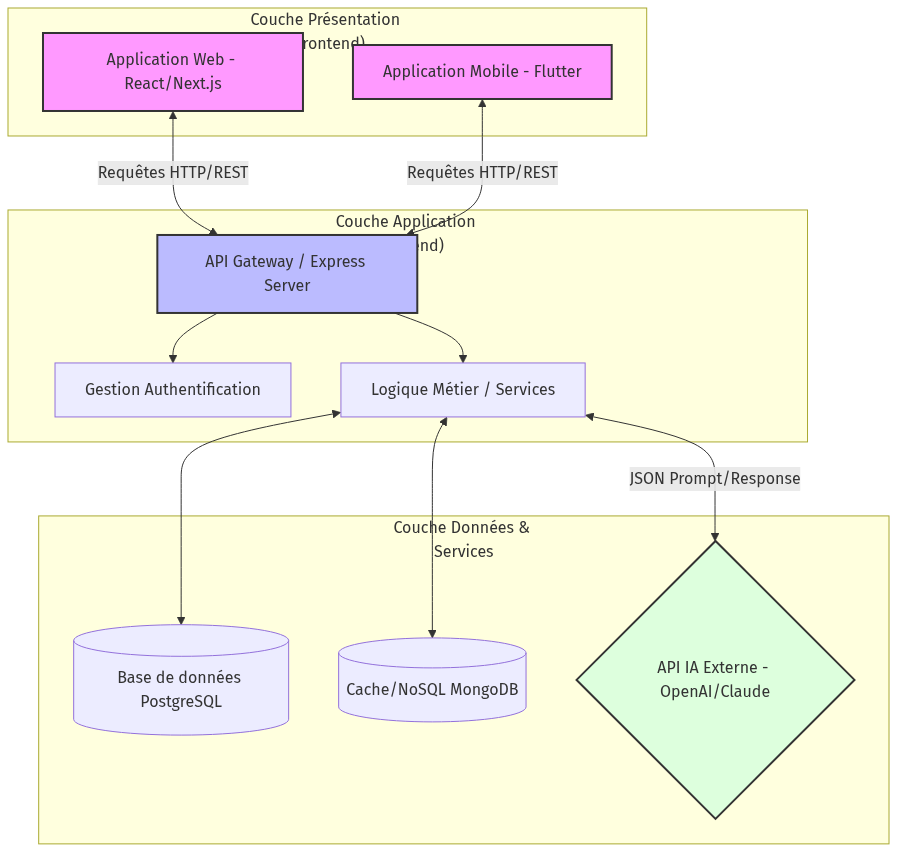
\includegraphics[width=0.9\textwidth]{arch_system.png}
    \caption{Architecture globale de l'application (Couches Présentation, Application et Données)}
\end{figure}

Ce diagramme illustre l'architecture fonctionnelle de la plateforme, divisée en trois couches principales qui garantissent la scalabilité, la sécurité et la modularité du système :
\begin{itemize}
    \item \textbf{La couche Présentation (Frontend)} : Héberge les interfaces de communication directe avec l'utilisateur, notamment l'application Web (développée par exemple en React ou Next.js) et l'application mobile (en Flutter). Le choix de ces technologies se justifie par la nécessité d'offrir une expérience utilisateur réactive, fluide et multiplateforme (iOS/Android) avec une base de code unifiée ou optimisée. Elle s'occupe de l'affichage interactif des cours et des quiz générés.
    \item \textbf{La couche Application (Backend)} : Constitue le centre névralgique de traitement du système. Elle se compose d'une API Gateway chargée d'acheminer et d'équilibrer les requêtes entrantes, d'un module de gestion d'authentification robuste (pour sécuriser les accès étudiants/professeurs via des tokens), ainsi que des micro-services gérant la logique métier propre à l'assistance académique. Cette séparation stricte permet de faire évoluer la logique sans impacter l'interface visuelle.
    \item \textbf{La couche Données et Services} : Représente la zone de persistance et d'assistance externe. Elle intègre la base de données relationnelle (PostgreSQL) choisie pour assurer la cohérence des données structurées, et une base de données non relationnelle (MongoDB) parfaite pour stocker les profils d'apprentissage flexibles. Enfin, elle pilote l'interface de connexion avec des modèles d'intelligence artificielle externes.
\end{itemize}
L'ensemble de ces couches communique de manière fluide, asynchrone et standardisée via des requêtes HTTP/REST et des échanges de données structurés en format JSON.

\section{Base de données et Communication Cloud}
La structure du système s'inscrit au niveau d'un déploiement distribué.

\begin{figure}[H]
    \centering
    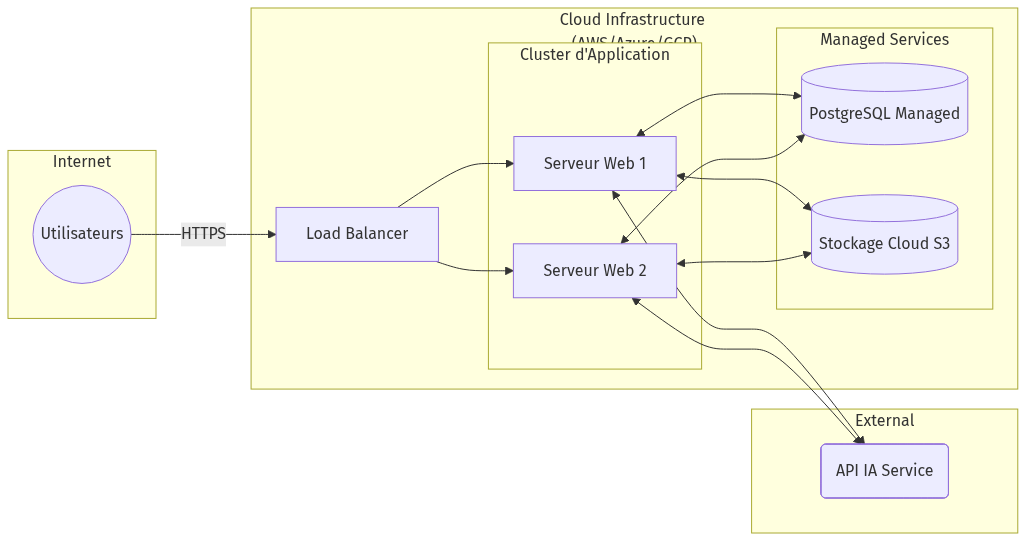
\includegraphics[width=0.9\textwidth]{deploy_diagram.png}
    \caption{Infrastructure et hébergement sur le Cloud}
\end{figure}

Ce diagramme détaille de manière approfondie la stratégie d'hébergement sur le Cloud, justifiée par la nécessité de garantir une haute disponibilité, une protection des données et une montée en charge fluide (scalabilité verticale et horizontale) lors de l'utilisation massive par les étudiants. On y retrouve :
\begin{itemize}
    \item \textbf{Une répartition de charge (Load Balancer)} : Placé en front-end de l'infrastructure Cloud, ce composant écoute le trafic HTTP/HTTPS entrant et distribue intelligemment les requêtes vers les différents serveurs du cluster. Cela évite la surcharge ponctuelle d'un serveur unique, critique en période de forts trafics (périodes d'examens).
    \item \textbf{Le Cluster d'Application} : Composé de plusieurs instances de serveurs (Serveurs Web Node.js ou équivalent), il assure la redondance : si un serveur Web tombe en panne, un autre prend instantanément le relais pour que l'application reste accessible sans aucune interruption de service ressentie par l'étudiant.
    \item \textbf{Les services infogérés (Managed Services)} : Les bases de données (comme PostgreSQL) et les espaces de stockage massif (Object Storage type S3 pour les cours ou les attestations en PDF) sont hébergés et gérés directement par le fournisseur cloud (AWS, Azure ou GCP). Ce choix soulage l'équipe de développement des tâches de maintenance complexes telles que les sauvegardes automatiques.
    \item \textbf{Interface API Externe de l'Intelligence Artificielle} : En aval, et de manière complètement décentralisée, nos serveurs métiers interrogent les services d'Intelligence Artificielle de manière sécurisée en tunnel chiffré, sans jamais exposer les clés API aux utilisateurs finaux naviguant sur l'application.
\end{itemize}

\section{Intégration d'une API d'intelligence artificielle}
Le diagramme de séquence ci-dessous décompose de manière exhaustive le processus clé de la plateforme : la génération intelligente d'exercices personnalisés. L'intégration de l'IA (Intelligence Artificielle) n'est pas effectuée en local pour des questions de ressources matérielles, mais est déportée via une API externe de traitement linguistique de grande envergure (Large Language Model - LLM). Le flux chronologique des actions est le suivant :
\begin{enumerate}
    \item \textbf{Action initiatrice de l'utilisateur} : L'étudiant clique sur le bouton de commande "Générer un Quiz" sur son interface (Frontend, web ou mobile). Cette action amorce le cycle de requête.
    \item \textbf{Interrogation sécurisée du Backend} : L'application Frontend compile une requête HTTP POST chiffrée, intégrant un jeton d'authentification valide (Token) pour prévenir l'usurpation d'identité, et y accole l'identifiant du cours souhaité, pour l'envoyer au Backend.
    \item \textbf{Extraction et compilation des ressources} : Le Backend réceptionne la commande, vérifie les droits d'accès, puis interroge la base de données relationnelle (PostgreSQL ou MongoDB) pour rapatrier le contenu textuel brut de la leçon ciblée ainsi que l'historique des notes et des faiblesses de l'étudiant concerné.
    \item \textbf{Génération par le modèle d'Intelligence Artificielle (API)} : Le composant métier du Backend synthétise intelligemment ces informations et façonne un "Prompt" (instruction contextuelle) optimisé. Il le transmet via l'API LLM (OpenAI, Mistral...) en y spécifiant le format de retour attendu. Le modèle d'intelligence artificielle analyse la requête et produit en temps réel des questions-réponses inédites ciblant les points faibles répertoriés de l'étudiant.
    \item \textbf{Validation, Sauvegarde et Restitution Interactive} : Le modèle distant renvoie les résultats structurés sous format JSON. Le Backend réceptionne cette réponse automatisée, valide son intégrité avant de l'ajouter dans la base de données au nom de l'étudiant pour assurer le suivi pédagogique continu. Il conclut le processus en retournant finalement le quiz généré au Frontend qui l'affichera sous une forme interactive de cartes ou questionnaires de révision.
\end{enumerate}

\begin{figure}[H]
    \centering
    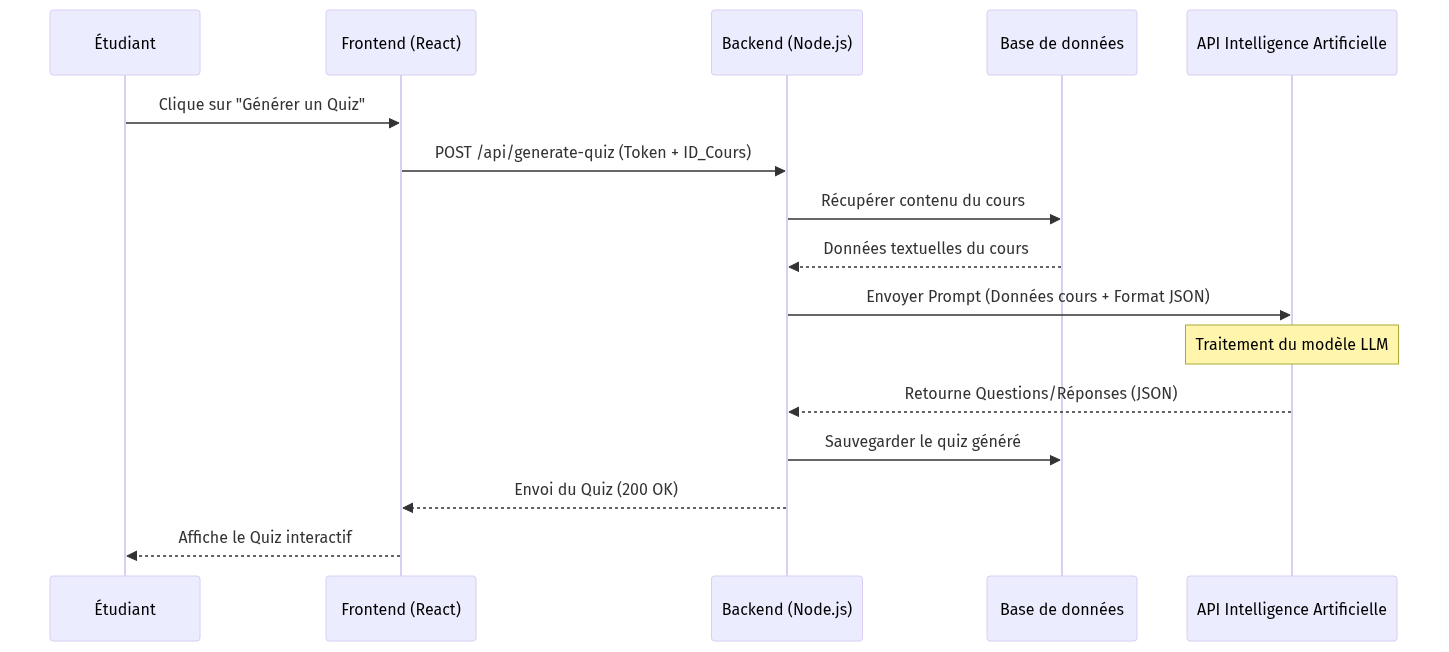
\includegraphics[width=0.9\textwidth]{seq_diagram.png}
    \caption{Diagramme de séquence pour la génération intelligente de quiz}
\end{figure}


\chapter{Gouvernance du projet et Conclusion}
\section{Organisation et Gestion des risques}
Toute contingence d'un ralentissement de programmation ou une erreur inattendue est préalablement discutée, de sorte à favoriser l'amélioration continue orientée CI/CD et l'assurance qualité avec le panel des étudiants.

\section{Conclusion}
Le projet présenté dans ce rapport propose la conception d'une plateforme numérique intelligente destinée à améliorer plusieurs aspects du fonctionnement universitaire. L'assistance numérique administrative couplée à un encadrement pédagogique par des algorithmes LLM récents garantit une solution viable et adaptée. L'objectif a donc été matérialisé par cette conception et offre un terrain porteur d'initiatives semblables pour moderniser la culture universitaire de demain.

\end{document}
